\documentclass[11pt, oneside]{article}
\usepackage[margin=1in]{geometry}
\geometry{letterpaper}
\usepackage{booktabs}
\usepackage{hyperref}
\usepackage{enumitem}
\usepackage{float}
\usepackage{caption}
\usepackage{subcaption}
\usepackage[numbers]{natbib}
\usepackage{graphicx}
\usepackage{amssymb}
\usepackage{amsmath}
\usepackage{array}
\usepackage{longtable}
\usepackage{xcolor}
\usepackage{tabularx}
\usepackage{setspace}
\usepackage{tikz}
\usetikzlibrary{arrows.meta,positioning}

\hypersetup{
    colorlinks=true,
    linkcolor=blue,
    citecolor=blue,
    urlcolor=blue
}
\captionsetup{font=small,skip=3pt}
\setlength{\textfloatsep}{8pt plus 2pt minus 2pt}
\setlength{\floatsep}{6pt plus 2pt minus 2pt}
\setlength{\intextsep}{6pt plus 2pt minus 2pt}

% ------------------------------------------------------------------------------------------------
% Author boxes: the course does not allow LLM-written analysis or conclusions.  Each box reserves
% roughly the space its text should take, so the page count of this draft matches the final report.
% Replace every box with your own prose before submission.
\definecolor{todo}{HTML}{FDF1E9}
\definecolor{todoline}{HTML}{EB6834}
\newcommand{\authorbox}[3]{\par\smallskip\noindent\fcolorbox{todoline}{todo}{\parbox[t][#3][t]{\dimexpr\linewidth-2\fboxsep-2\fboxrule}{%
  \footnotesize\textbf{To be written by the author --- #1.}\ #2}}\par\smallskip}
\newcommand{\fillin}{\rule{1.2cm}{0.4pt}}
\newcommand{\code}[1]{\texttt{\small #1}}

% ============================================================
% TITLE BLOCK --- students must keep this format
% Replace placeholders. Do not redesign the title page.
% Filename of the compiled PDF must be:
% CS781-CP-[Firstname]-[Lastname]-[RollNo]-report.pdf
% ============================================================
\title{CS781 Capstone Project:\\
In-House Legal Intelligence System}
\author{
    Manish Kumar  \\
    251330604 \\
    {\tt \{manishkmr25\}@iitk.ac.in}\\
    Indian Institute of Technology Kanpur (IIT Kanpur)
}
\date{}

\begin{document}
\maketitle

\begin{abstract}
Imagine a law firm that wants AI help with its case files but cannot let a single page leave the building.
That was our brief.  We built everything ourselves: four small legal language models (82--89M parameters)
trained from scratch on Indian court and legislative text, and six tools on top of them that find named
entities, label the role of each sentence, predict case outcomes, identify statutes, write summaries and
retrieve prior cases.  Along the way we found that the starter data leaked validation text and was full of
duplicates and OCR noise; cleaning it cut A4's perplexity from 13.3 to 11.3 at the same budget.  The biggest
gains came from respecting how legal documents are built: reading the end of a judgment for its outcome
(0.754 to 0.785), and matching each citation on its own when retrieving precedents (0.32 to 0.43).
\end{abstract}

% ============================================================
\section{Competition Result}
% ============================================================
\noindent
\textbf{Codabench username:} m\_251330604
\hfill
\textbf{Roll number:} 251330604\\
\textbf{GitHub repository:} \url{https://github.com/manishkr21/capstone_llm}

\medskip
\noindent
Here is where we stood on the leaderboard when we froze the report.

\begin{table}[H]
\centering
\caption{Official phase scores and ranks. Fill every cell. State the date on which ranks were recorded.}
\label{tab:leaderboard}
\small
\begin{tabular}{clccc}
\toprule
Phase & Task & Primary metric (value) & Rank & Valid submissions \\
\midrule
1 & Legal LM Pretraining & BERTScore F1: 0.8286 & 95 & 6 \\
2 & Legal NER & strict macro-F1: 0.4970 & 80 & 6 \\
3 & Rhetorical role prediction & macro-F1: 0.5750 & 15 & 51 \\
4 & Court judgment prediction & macro-F1: 0.8121 & 13 & 30 \\
5 & Legal statute identification & macro-F1: 0.4624 & 6 & 50 \\
6 & Abstractive summarization & BERTScore F1: 0.8558 & 4 & 32 \\
7 & Prior case retrieval & micro-F1@7: 0.4950 & \fillin & 21 \\
\bottomrule
\end{tabular}
\end{table}

\noindent
\textbf{Total valid Codabench submissions across all phases:} 196
\quad
\textbf{Date ranks were recorded:} 6 November 2026

\medskip
\noindent We cleared the minimum of four distinct submissions in every phase (six or more each); the six best
of each phase, and what produced them, are listed in \autoref{app:top6}.

% ============================================================
\section{Introduction and Problem Description}
% ============================================================
Law firms sit on mountains of text, and most of it is confidential.  A firm that wants language technology
therefore cannot simply call a commercial API, and it cannot fine-tune someone else's foundation model whose
data and licence it does not control.  The capstone turns this into a concrete challenge: train your own
compact language model (50--300M parameters, no pretrained weights, only the official
\texttt{Exploration-Lab/CS-781-Capstone} data), then teach it six real legal tasks taken from the IL-TUR
benchmark \cite{joshi2024iltur}.  \autoref{tab:tasks} lists them.

\begin{table}[!t]\centering\footnotesize
\caption{Tasks (inputs, outputs and primary metrics as scored on Codabench).}\label{tab:tasks}
\scriptsize\begin{tabularx}{\linewidth}{clXl}\toprule
Ph. & Task & Input $\rightarrow$ output & Primary metric\\\midrule
1 & Legal LM & 512-word legal prompt $\rightarrow$ 128-word continuation & BERTScore F1\\
2 & L-NER & judgment text $\rightarrow$ character spans with one of 12 entity types & strict macro-F1\\
3 & Rhetorical roles & sentences of a judgment $\rightarrow$ one of 13 roles each (Corporate Law, IT) & macro-F1\\
4 & Judgment prediction & judgment (outcome removed) $\rightarrow$ allowed (1) / dismissed (0) & macro-F1\\
5 & Statute identification & case text (statute names masked) $\rightarrow$ set of statute ids (of 100) & macro-F1\\
6 & Summarization & judgment $\rightarrow$ abstractive summary & BERTScore F1\\
7 & Prior case retrieval & query judgment + candidate pool $\rightarrow$ 7 ranked case ids & micro-F1@7\\
\bottomrule\end{tabularx}\end{table}

Three things made this harder than it sounds.  Legal documents are \emph{long}: a typical judgment runs to
thousands of words (median 2,469 tokens in Phase~4, 4,508 words in Phase~7), while our models can only look at
1,024 tokens at a time.  The \emph{metrics are unforgiving}: an entity counts only if every character matches,
rare classes weigh as much as common ones, and a summary is compared with a single reference.  And we had
\emph{one GPU}, shared with other people's jobs.

So we kept asking the same few questions.  Does cleaning the data matter more than the architecture?  How well
do our small models carry over to each task?  Can cheap adaptation methods match full fine-tuning?  How do you
feed a 20-page judgment to a model that reads two pages?  And how much do decoding and threshold choices move
the score?  We built and submitted every phase end to end.  We did not chain the phases together, train a
separate tokenizer per task, or have lawyers judge the outputs.

% ============================================================
\section{Data Analysis and Preprocessing}
% ============================================================
\subsection{Sources and official splits}
We used only the official dataset.  \autoref{tab:data} shows what each phase looked like after we cleaned it,
and the numbers that ended up shaping our design.

\begin{table}[!t]\centering\footnotesize
\caption{Data per phase as used (after de-duplication and leak removal).  Lengths are medians.}\label{tab:data}
\scriptsize\begin{tabularx}{\linewidth}{clX}\toprule
Ph. & Split sizes & Statistics that informed the design\\\midrule
1 & 1.006B train tokens (cleaned), 4.10M val tokens & 3.48M documents read; 106,717 exact and 204,246 near
duplicates removed; 90,856 documents with OCR word stutter repaired; 764 validation documents dropped as leaks\\
2 & 70 train docs (10 held out), 35 test & 8,393 entities in 12 types; median 4,488 words per document\\
3 & 90 labelled docs (45 CL, 45 IT), 10 test & labels persist: next sentence has the same role with
probability 0.94 (CL) / 0.75 (IT); PrecedentOverruled has 3 training sentences\\
4 & 31,677 train, 1,988 clean val, 1,517 test & 58.6\% of training labels are 0, validation and test balanced;
median 2,469 tokens (train), 3,771 (val)\\
5 & 42,315 train, 10,024 val, 13,019 test & 100 statutes, 3.71 per document; frequency 270--11,577 documents;
statute names masked as \code{<SECTION>}/\code{<ACT>}\\
6 & 6,703 train, 300 val (ours), 100 test & documents 3,123 words, summaries 640 words (compression 4.6);
75\% of references exceed the $\approx$400 words that BERTScore compares\\
7 & 827 / 118 / 237 queries; pools 4,320 / 1,023 / 1,727 & 6.4--8.2 gold cases per query (range 0--92);
citations masked as \code{<CITATION>}; a perfect 7-item list scores only 0.618 on dev\\
\bottomrule\end{tabularx}\end{table}

\paragraph{Surprises in the data.}  Before training anything, we checked the files, and they were not always
what they seemed.  The Phase-1 starter split had validation documents copied into training, so we built a
fresh validation set that shares no text with either corpus.  In Phase~4 the test file still contained its
labels, and every test document also appeared, labelled, in the development file; we never read those labels
and chose models only on the 1,988 development documents not in the test set.  In Phase~5 we removed
development texts that also sat in the test file (96) or in training (118), and merged 435 duplicates.  Phase~7
had the most interesting quirk: every query appears in its own candidate pool, and almost every other case in
a pool (99.9\% on train, 100\% on dev) is the correct answer for \emph{some} query.  We used that later.

\begin{figure}[!t]\centering
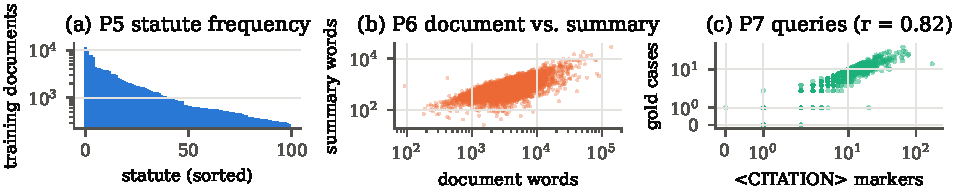
\includegraphics[width=\linewidth]{figs/data.pdf}
\caption{(a) Phase-5 statutes per training document count, sorted (log scale).  (b) Phase-6 document length
against summary length.  (c) Phase-7 training queries: number of \code{<CITATION>} markers against number of
gold cases.}\label{fig:data}
\end{figure}

\subsection{Preprocessing decisions}
Every model shares one byte-level BPE tokenizer \cite{sennrich2016bpe} with 32,000 tokens, trained on legal text,
so Devanagari names, section symbols and OCR debris never turn into ``unknown''.  Cleaning the Phase-1 corpus
meant normalising characters, repairing OCR stutter (``the the the court''), dropping short or garbled
documents, and removing exact and near-duplicates.  NER needed special care because a single character off
means a miss: we split runs of punctuation before tokenizing and kept a map from every token back to its
characters, so spans survive the round trip (99.45\% exactly, up from 98.66\%).  For long documents each phase
found its own trick: read eight 512-token chunks (the \emph{last} eight for outcomes), condense a judgment to
its opening plus its most central sentences for summaries, or cut out the $\pm60$ words around each citation
for retrieval.

% ============================================================
\section{Approach and Model Evolution}
% ============================================================
\subsection{Phase-1 foundation model}
We built four quite different models and trained them identically, so that any difference comes from the
architecture alone (\autoref{tab:arch}).  All learn to predict the next word on 1,024-token windows; the
encoder--decoder learns to continue a random-length prefix, and the prefix-LM reads part of its input in both
directions.  Our first models (R0) used the starter sample of about 200M tokens.  After the data audit we
retrained them on the cleaned corpus at the same budget (R1), then kept going to 1B tokens (R2).  For the
submission, text is sampled with temperature 0.8, top-$k$ 50, top-$p$ 0.95 and a mild repetition penalty
\cite{keskar2019ctrl}, and the model is not allowed to stop before 128 words.

\begin{table}[!t]\centering\footnotesize
\caption{The four Phase-1 architectures (vocabulary 32k, context 1,024).}\label{tab:arch}
\begin{tabularx}{\linewidth}{lXr}\toprule
ID & Design & Params\\\midrule
A1 & Decoder-only \cite{radford2019gpt2}; learned positions, pre-LayerNorm, GELU; 8 layers, $d=768$, 12 heads, $d_\text{ff}=3072$ & 82.1M\\
A2 & Encoder--decoder \cite{vaswani2017attention}, 6+6 layers, sinusoidal positions, $d=640$, 10 heads & 89.4M\\
A3 & Prefix-LM: bidirectional prompt, causal continuation, ALiBi \cite{press2022alibi}; 8 layers, $d=768$ & 81.3M\\
A4 & RoPE \cite{su2021roformer}, RMSNorm, SwiGLU, grouped-query attention \cite{ainslie2023gqa} (12 q / 4 kv heads),
256-token sliding window \cite{beltagy2020longformer} with every third layer global; 10 layers, $d=768$ & 87.5M\\
\bottomrule\end{tabularx}\end{table}

\subsection{Transfer protocol (Phases 2--7)}
From here on, every task model starts from one of our Phase-1 checkpoints and learns only from that task's
data (\autoref{fig:system}).  A small wrapper turns each language model into an encoder.  We learned along the
way that A1 and A4 work best when they keep their original left-to-right attention, that A3 should read its
input in both directions, and that A2's encoder had collapsed during pre-training, so we use its decoder
instead.  We wrote each adaptation method once and reused it everywhere: full and partial fine-tuning, gradual
unfreezing \cite{howard2018ulmfit}, BitFit \cite{benzaken2022bitfit}, LoRA \cite{hu2022lora}, LoRMA
\cite{bihany2025lorma}, QLoRA \cite{dettmers2023qlora}, AdaLoRA \cite{zhang2023adalora}, Houlsby adapters
\cite{houlsby2019adapters}, IA$^3$ \cite{liu2022ia3}, prefix \cite{li2021prefix} and prompt tuning
\cite{lester2021prompt}, and knowledge distillation \cite{hinton2015kd} into smaller students.  Every phase
tried at least six of them, across all four architectures.

\begin{figure}[!t]\centering
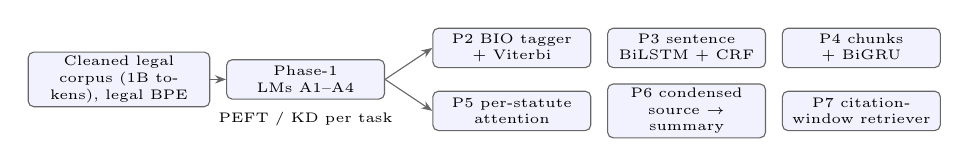
\begin{tikzpicture}[node distance=2mm, box/.style={draw=black!60,rounded corners=2pt,fill=blue!5,align=center,
  font=\tiny,minimum height=5mm,text width=19mm,inner sep=1.5pt}, arr/.style={-{Stealth[length=1.4mm]},black!60}]
  \node[box,text width=22mm] (c) {Cleaned legal corpus (1B tokens), legal BPE};
  \node[box,right=of c] (b) {Phase-1 LMs A1--A4};
  \node[box,right=6mm of b,yshift=4mm] (t1) {P2 BIO tagger + Viterbi};
  \node[box,right=of t1] (t2) {P3 sentence BiLSTM + CRF};
  \node[box,right=of t2] (t3) {P4 chunks + BiGRU};
  \node[box,right=6mm of b,yshift=-4mm] (t4) {P5 per-statute attention};
  \node[box,right=of t4] (t5) {P6 condensed source $\rightarrow$ summary};
  \node[box,right=of t5] (t6) {P7 citation-window retriever};
  \draw[arr] (c)--(b); \draw[arr] (b.east)--(t1.west); \draw[arr] (b.east)--(t4.west);
  \node[font=\tiny,below=0.3mm of b,text width=24mm,align=center] {PEFT / KD per task};
\end{tikzpicture}
\caption{One pre-trained backbone family, six separately fine-tuned descendants.}\label{fig:system}
\end{figure}

\subsection{Phase 2 --- Legal NER}
We turned entity spans into B/I/O tags on tokens, let each backbone tag overlapping 512-token windows (each
token trusts the window where it sits most centrally), and decoded with a Viterbi pass that refuses impossible
tag sequences, before mapping tags back to exact characters.  Six experiments covered all four architectures.

\subsection{Phase 3 --- Rhetorical role prediction}
A sentence's role depends on its neighbours, and roles come in long runs, so we never classify a sentence
alone.  Neighbouring sentences are encoded together, each sentence is pooled into one vector, a BiLSTM reads
the whole document, and a CRF \cite{lafferty2001crf} picks the most plausible sequence of roles.  Corporate
Law and IT share one model with a domain flag; rare roles get extra weight through logit adjustment; and with
only 90 labelled documents, everything is judged by five-fold cross-validation.

\subsection{Phase 4 --- Court judgment prediction}
A judgment is cut into 512-token chunks; the model reads eight of them, summarises each, and lets a BiGRU with
attention \cite{yang2016han} decide which chunks matter.  Training data leans 59/41 towards dismissals while the
test set is balanced, so we weighted the loss and tuned the decision threshold on validation.  The metric is
macro-F1 rather than accuracy, so that ``allowed'' and ``dismissed'' count equally.

\subsection{Phase 5 --- Legal statute identification}
Statutes are usually discussed in one part of a judgment, so we gave each of the 100 statutes its own
attention query: it looks for the chunks that talk about it.  Rare statutes get larger loss weights
($\sqrt{n_\text{neg}/n_\text{pos}}$, capped at 30) and their own decision thresholds.  Later we trained
6-block students to imitate ensembles of our best runs, and finally combined all runs with MLP and per-statute
LightGBM \cite{ke2017lightgbm} stackers, optionally adding simple TF-IDF models (a hybrid that uses no
pretrained weights).

\subsection{Phase 6 --- Abstractive summarization}
Here the model reads [a short prompt, the condensed judgment, ``\texttt{Summary:}''] and learns to write the
summary; A2 reads four chunks separately and fuses them in its decoder \cite{izacard2021fid}.  Since a summary
can only mention what the model has read, we kept stretching the input: stretching A1's position table
\cite{chen2023pi} let sources grow from 1,280 to 8,192 tokens, each step starting from the previous model.
Decoding is greedy with a repetition penalty and no repeated 3-grams.  As a final step we can pick, for each
document, the candidate summary that agrees most with the others (minimum-Bayes-risk selection
\cite{kumar2004mbr}).

\subsection{Phase 7 --- Prior case retrieval}
Each \code{<CITATION>} marker in a query hides one cited case, and the words around it describe that case.
So instead of matching the whole judgment, we search with each citation's neighbourhood separately using
BM25 \cite{robertson2009bm25}, push down cases decided after the query, and use the pool quirk above: since
every case in the pool is cited by \emph{someone}, we also ask which query each case fits best.  On top sits a
neural retriever built on a Phase-1 model, trained with InfoNCE \cite{oord2018cpc} against hard negatives
from BM25, and a LightGBM ranker that re-orders the top 100 candidates using both.

\subsection{Final submitted system}
\begin{table}[!t]\centering\footnotesize
\caption{Best Codabench submission per phase, its checkpoint(s) and local held-out score.}\label{tab:final}
\begin{tabularx}{\linewidth}{clXrr}\toprule
Ph. & Submission & Checkpoint(s) & Local & Codabench\\\midrule
1 & A1 R0 & \code{runs/A1\_gpt/best1.pt} (starter corpus, 200M tokens) & 0.829 & 0.8286\\
2 & E2 & A4 LoRMA on \code{runs/A4\_efficient/best.pt}, BIO Viterbi & 0.486 & 0.4970\\
3 & T14 & A1 LoRA, causal, 1,024-token windows, 5 fold models & 0.501 & 0.5750\\
4 & STACK\_with\_fusion & logistic-regression stacker over 26 runs (\autoref{app:top6}) & 0.823 & 0.8121\\
5 & STACK11\_full & MLP + LightGBM stackers, 28 Phase-1 + 6 lexical models & 0.460 & 0.4624\\
6 & S3 beam 4 & A4 full fine-tuning, 4,096-token source, 4 beams & 0.852 & 0.8558\\
7 & STK4 & LightGBM re-ranker + mean of 4 bi-encoders & 0.491 & 0.4950\\
\bottomrule\end{tabularx}\end{table}

% ============================================================
\section{Experiments and Implementation Details}
% ============================================================
\subsection{Compute and training protocol}
Everything ran on one NVIDIA H200 that we shared with other people's jobs, so we could rarely run more than
two to four experiments at once.  The longest Phase-1 run took about an hour per architecture for 803M tokens;
task runs took anywhere from 2 minutes to 3.5 hours.  All of them used AdamW with warm-up and cosine decay,
gradient clipping and bf16, saved their best state, and could resume after a crash.

\begin{table}[!t]\centering\footnotesize
\caption{Hyperparameters of the final model of each phase (P5--P7: the best single Phase-1 model).
$^*$R2, after 3,000 steps of R1.}\label{tab:hparams}
\resizebox{\linewidth}{!}{\begin{tabular}{lccccccc}\toprule
Hyperparameter & P1 (A4) & P2 (A4 LoRMA) & P3 (A4 LoRMA) & P4 (A4 partial) & P5 (A4 KD) & P6 (A1 full) & P7 (A1 full)\\\midrule
Parameters (M) & 87.5 & 87.5 (2.2 trained) & 87.5 & 88.0 (25.7 tr.) & 63.4 & 85.0 & 82.3\\
Context length & 1,024 & 512 windows & 512 windows & 8$\times$512 & 8$\times$512 & 4,096 + 768 & 256 / 512\\
Peak LR & $6\!\times\!10^{-4}$ & $10^{-3}$ & $10^{-3}$ & $10^{-4}$ & $5\!\times\!10^{-5}$ & $5\!\times\!10^{-5}$ & $3\!\times\!10^{-5}$\\
Batch $\times$ accum. & 8 $\times$ 8 seq. & 16 windows & 4 chunks & 2 $\times$ 8 docs & 4 $\times$ 4 docs & 1 $\times$ 16 & 8 queries\\
Epochs / steps & 12,260 steps$^*$ & $\le$15 (patience 5) & 20 (patience 6) & 2 & 8 & 3 (+6 at 2,560) & 10 (best 5)\\
Dropout & 0 & 0.1 & 0.1 & 0.1 & 0.1 & 0.1 & 0\\
Decoding / threshold & $T$ 0.8, top-$p$ 0.95 & BIO Viterbi & CRF Viterbi & 0.39 & per statute & greedy, pen.\ 1.15 & top 7\\
\bottomrule\end{tabular}}\end{table}

\subsection{Local evaluation}\label{sec:localeval}
Because Codabench only shows a score after you upload, we needed honest local scores first.  Each phase got
its own held-out set built from public data: a leak-free Phase-1 validation set, 10 held-out NER documents
(double-checked on three splits), five-fold cross-validation in Phase~3, the development documents not in the
test set in Phase~4, cross-fitted thresholds in Phase~5, 300 held-out documents in Phase~6, and the official
dev split in Phase~7.  A script checked every zip before upload, catching missing ids, wrong counts and
duplicate answers.  Local and leaderboard scores do not always agree, partly because some local sets are small
and partly because we score summaries with roberta-large while the organisers use a ``legal BERTScore''.

\subsection{Ablations and controlled comparisons}
To know what actually helped, we changed one thing at a time.  Each row of \autoref{tab:ablations} compares
two runs that differ only in the factor named.

\begin{table}[!t]\centering\footnotesize
\caption{One-factor comparisons on the local held-out split of each phase.  $^\dagger$Three changes at once:
causal mask, 20 epochs, logit adjustment $\tau=0.5$.  OOF = out-of-fold, CF = cross-fitted.}\label{tab:ablations}
\scriptsize\begin{tabularx}{\linewidth}{cXlrr}\toprule
Ph. & Factor changed (everything else fixed) & Model, metric & Before & After\\\midrule
1 & Corpus cleaning, same 200M tokens & A4, fair-val perplexity & 13.32 & 11.25\\
1 & Token budget 200M $\rightarrow$ 1B & A4, fair-val perplexity & 11.25 & 8.26\\
2 & Argmax $\rightarrow$ BIO Viterbi decoding & A4 LoRMA, macro-F1 & 0.373 & 0.486\\
2 & Original $\rightarrow$ cleaned 1B backbone & A4 LoRMA, macro-F1 (3 splits) & 0.488 & 0.467\\
3 & Sentence alone $\rightarrow$ context window & A4 LoRMA, OOF macro-F1 & 0.361 & 0.455\\
3 & Tuning round$^\dagger$ & A4 LoRMA, OOF macro-F1 & 0.455 & 0.500\\
4 & First 8 $\rightarrow$ last 8 chunks & A4 partial, macro-F1 & 0.754 & 0.785\\
5 & 3 $\rightarrow$ 5 epochs & A4 partial, CF macro-F1 & 0.370 & 0.381\\
5 & Spread $\rightarrow$ statute-placeholder chunks & A4 partial, CF macro-F1 & 0.370 & 0.371\\
5 & KD teacher 5 $\rightarrow$ 8 models & 6-block A4 student, CF macro-F1 & 0.404 & 0.402\\
6 & Repetition penalty + no repeated 3-grams & 9 first-round runs, BERTScore & \multicolumn{2}{r}{+0.003 to +0.008}\\
6 & Source 1,280 $\rightarrow$ 2,560 tokens & A1 full, BERTScore F1 & 0.8505 & 0.8520\\
6 & Spread $\rightarrow$ salient condensation & A1 LoRA, BERTScore F1 & 0.8452 & 0.8493\\
7 & Whole query $\rightarrow$ per-citation BM25 & no learning, micro-F1@7 & 0.324 & 0.432\\
7 & + case-wise pool normalisation & BM25 + date penalty, micro-F1@7 & 0.453 & 0.469\\
7 & No teacher $\rightarrow$ distillation from E2 & 4-block A1, neural micro-F1@7 & 0.354 & 0.369\\
\bottomrule\end{tabularx}\end{table}

% ============================================================
\section{Results}
% ============================================================
\autoref{tab:variants} puts our local scores next to the leaderboard, and \autoref{fig:curves} and
\autoref{fig:perclass} show how training went.  Averages hide a lot: two Phase-3 roles have almost no training
examples (3 sentences for PrecedentOverruled, 2 documents for Dissent), and in Phase~5 the rarest fifth of
statutes averages 0.32 F1 against 0.56 for the most common.

\begin{table}[!t]\centering\footnotesize
\caption{Main variants: local held-out score next to the Codabench test score (-- = not uploaded).  Secondary
(local): P1 ROUGE-L/BLEU-4, P2 and P4 precision/recall, P5 micro-F1, P6 ROUGE-1/ROUGE-L, P7 precision/recall.}\label{tab:variants}
\scriptsize\begin{tabularx}{\linewidth}{clXrrr}\toprule
Ph. & Variant & Detail & Local & Secondary & Codabench\\\midrule
1 & A1 R0 & starter corpus, 200M tokens & 0.829 & 0.192 / 0.058 & 0.8286\\
1 & A4 R0 & starter corpus, 200M tokens & 0.827 & 0.186 / 0.050 & 0.8280\\
1 & A4 R2 & cleaned, 1B tokens & 0.836 & 0.213 / 0.093 & --\\
2 & E2 A4 LoRMA & 2.2M trained parameters & 0.486 & 0.517 / 0.478 & 0.4970\\
2 & E1 A3 full & full fine-tuning & 0.427 & 0.447 / 0.441 & 0.4815\\
2 & E6 KD student & 4-block A3, 52.9M parameters & 0.344 & 0.372 / 0.344 & 0.3799\\
3 & T7 A4 LoRMA & tuned, out-of-fold & 0.500 & -- & 0.5586\\
3 & T14 A1 LoRA & tuned, 1,024-token windows & 0.501 & -- & 0.5750\\
3 & C7 ensemble & 8 taggers, out-of-fold & 0.521 & -- & 0.5707\\
4 & E6 A4 partial & best single model & 0.785 & 0.787 / 0.786 & 0.7633\\
4 & ENS\_top5 & mean of 5 runs & 0.797 & 0.800 / 0.798 & 0.7930\\
4 & STACK\_with\_fusion & stacker, nested estimate & 0.823 & -- & 0.8121\\
5 & STACK6 & stacker, Phase-1 runs only & 0.423 & 0.520 & 0.4231\\
5 & STACK11 & hybrid stacker (+ TF-IDF) & 0.460 & 0.558 & 0.4624\\
6 & F1 A4 full & 1,280-token source, first decode & 0.843 & 0.477 / 0.251 & 0.8483\\
6 & S7 A1 full & 4,096-token source, greedy & 0.854 & 0.513 / 0.273 & 0.8508\\
6 & S3 A4 full & 4,096-token source, beam 4 (100 docs) & 0.852 & 0.525 / 0.275 & 0.8558\\
7 & STK0 & lexical re-ranker only & 0.477 & 0.519 / 0.441 & 0.4725\\
7 & E2 A1 full & bi-encoder fused with BM25 & 0.470 & -- & 0.4643\\
7 & STK4 & re-ranker + 4 bi-encoders & 0.491 & 0.535 / 0.454 & 0.4950\\
\bottomrule\end{tabularx}\end{table}

\begin{figure}[!t]\centering
\begin{subfigure}{0.49\linewidth}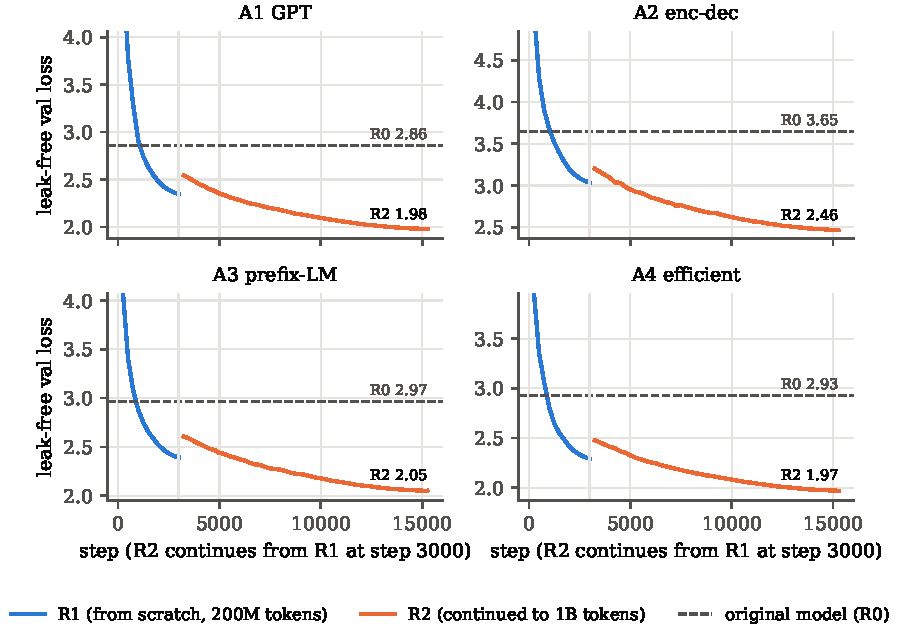
\includegraphics[width=\linewidth,height=2.4cm,keepaspectratio]{figs/p1_val_retrain.pdf}\caption{Phase 1: validation loss against training tokens.}\end{subfigure}\hfill
\begin{subfigure}{0.49\linewidth}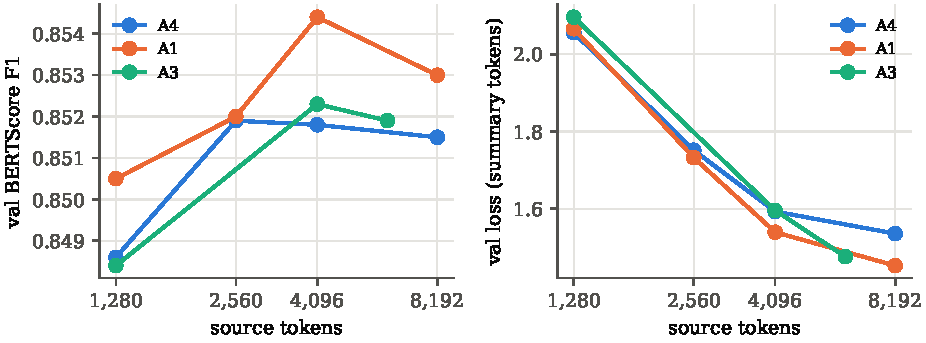
\includegraphics[width=\linewidth,height=2.4cm,keepaspectratio]{figs/p6_source_length.pdf}\caption{Phase 6: BERTScore and loss against source length.}\end{subfigure}
\caption{Learning curves and the source-length experiment.}\label{fig:curves}
\end{figure}

\begin{figure}[!t]\centering
\begin{subfigure}{0.45\linewidth}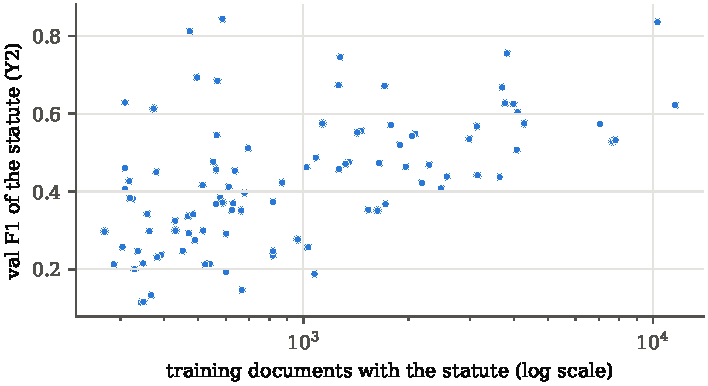
\includegraphics[width=\linewidth,height=3.6cm,keepaspectratio]{figs/p5_perlabel.pdf}\caption{Phase 5: per-statute F1 (best single model) against training frequency.}\end{subfigure}\hfill
\begin{subfigure}{0.53\linewidth}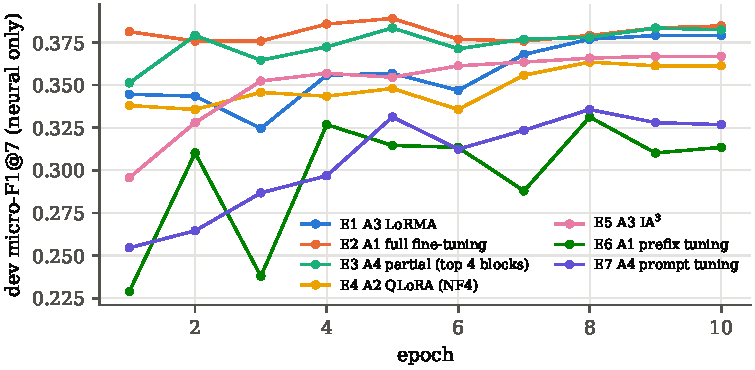
\includegraphics[width=\linewidth,height=3.6cm,keepaspectratio]{figs/p7_curves.pdf}\caption{Phase 7: dev micro-F1@7 of the bi-encoders after each epoch.}\end{subfigure}
\caption{Per-class breakdown (Phase 5) and task metric against epochs (Phase 7).}\label{fig:perclass}
\end{figure}

\paragraph{Which system won, and why.}  The winners differ by phase, but the reasons repeat.  In
\textbf{Phase~1}, A1, A3 and A4 finish within 0.0006 of each other on Codabench, while A2 trails (0.8184): with
the same data and budget, the decoder-style models are interchangeable, and the encoder--decoder pays for
splitting its capacity between two stacks (its encoder output later turned out to be nearly constant).  In
\textbf{Phase~2}, A4 with LoRMA won with only 2.2M trained parameters.  With 70 training documents, updating a
small multiplicative correction preserves what pre-training learned better than rewriting all weights, and
the constrained decoder mattered even more than the backbone (argmax 0.373 vs.\ Viterbi 0.486).  In
\textbf{Phase~3}, the winner (A1 LoRA with 1,024-token windows) is the variant that sees the most neighbouring
sentences; adding context was the single largest change we measured (0.361 to 0.455), because roles are defined
by where a sentence sits in the argument.  In \textbf{Phase~4}, the stacker won because its members read
different parts of the judgment (last, first, spread chunks) and therefore make different mistakes, and the
end of the judgment, where the outcome is argued, carries most of the signal (0.785 vs.\ 0.754).  In
\textbf{Phase~5}, the hybrid stack beat the Phase-1-only stack (0.462 vs.\ 0.423 on Codabench): statute names are
masked, but TF-IDF models still pick up exact phrases that accompany a statute (offence wording, procedural
terms) across the whole document, which eight 512-token chunks cannot all cover, so the two families err on
different documents.  In \textbf{Phase~6}, longer sources won (1,280 to 2,560 tokens: +0.0015), since a
summary cannot mention what the model never read, and beam search helped more on Codabench (0.8558 vs.\ 0.8520
greedy) than locally.  In \textbf{Phase~7}, most of the score comes from matching each citation separately and
from normalising across the pool (0.324 to 0.483 with no learning); the Phase-1 retrievers add about 0.01--0.02
on top by recognising paraphrased legal reasoning that word overlap misses.

% ============================================================
\section{Error Analysis and Discussion}
% ============================================================
\subsection{Phase-wise failure modes}
Every phase fails in a way that tells us something about legal text.  In \textbf{NER}, the problem is mostly
silence rather than confusion: 37.9\% of gold entities are never predicted, against 8.0\% with a wrong boundary
and 5.6\% with a wrong type.  Strict span matching turns any boundary slip into a miss, and the commonest type
error, appellant tagged as respondent (35 cases), is one that a 512-token window cannot resolve, because who is
the appellant is settled pages earlier.  In \textbf{rhetorical roles}, the model mixes up Ratio and
PrecedentRelied (548 and 539 sentences) and Fact and Ratio (499).  These sentences use the same vocabulary; what
differs is \emph{whose} reasoning it is, a discourse cue the sentence encoder only partly sees.  Roles with three
training sentences are simply never learned.  In \textbf{judgment prediction}, errors are fairly balanced (176
false positives, 250 false negatives), and reading the last chunks instead of the first (0.785 vs.\ 0.754)
supports the idea that the outcome is argued near the end.  In \textbf{statute identification}, the most common
error is telling: a missed statute is replaced by the most frequent one, so when evidence is weak the model falls
back on its prior, and rare statutes suffer (mean F1 0.32 for the rarest fifth, 0.56 for the most frequent).  In
\textbf{summarization}, scores fall as judgments get longer (correlation $-0.40$): condensation has to drop more,
and whatever it drops cannot appear in the summary.  In \textbf{retrieval}, 8 of 118 dev queries get no correct
case, and queries citing only one to three cases are capped by the fixed list of seven (precision 0.21).

\subsection{What the metrics do not measure}
None of these numbers checks legal correctness.  A summary can score a high BERTScore while stating the wrong
holding, because embedding similarity rewards shared vocabulary, and only its first $\approx$400 words are
compared at all.  Strict span-F1 counts an entity as wrong when one character is off, which is harsher than a
lawyer would be, while micro-F1@7 forces seven answers even when a case cites one.  For a firm, this means every
output should be treated as a draft with a confidence attached, never as a final answer.

\subsection{Limitations and what you would do next}
We trained on one shared GPU, so most runs have a single seed, and our validation sets are small (118 queries,
300 summaries), which makes differences below about 0.015 noise.  The Phase-1 models never saw more than 1,024
tokens, yet Phases 4--7 run them on documents several times longer.  We had no human legal evaluation, and two
of our best systems (Phases 5 and 7) lean on lexical models.  With more time we would continue pre-training the
cleaned A4 model at 4,096 tokens, resolve party roles at the document level for NER, and pre-train the retriever
on citation contexts mined from the Phase-1 corpus itself.

\subsection{Surprising findings}
Three results went against our expectations.  The cleaned corpus lowered perplexity everywhere, yet NER got
slightly worse with the new backbone (0.488 to 0.467).  In Phase~7, the largest gains came from the structure of
the data (one query per citation, normalising scores across the pool), not from the neural model.  And local
and leaderboard rankings did not always agree: in Phase~3 a single model beat our ensembles on Codabench.

% ============================================================
\section{Conclusion}
% ============================================================
We delivered what the brief asked for: four legal language models trained from scratch and six task systems
built on them, all running on in-house hardware with no outside data or services.  What moved the metrics was
mostly how we handled the documents (cleaning the corpus, reading the end of a judgment, feeding longer
sources, retrieving per citation) and combining models, while the choice among architectures and adaptation
methods mattered less, with LoRMA and partial fine-tuning close to full fine-tuning.  The main lesson is that a
small model gains more from understanding the shape of legal text than from extra parameters.  A sceptical
partner should still not trust the summaries without reading the judgment, should expect the retriever to miss
about half of the cited cases, and should know that NER misses roughly a third of entities.

\clearpage
% ============================================================
\section*{LLM Usage Declaration}\label{sec:llm}
% ============================================================
Completing this section is mandatory. Inconsistent answers relative to the code and the prose will be treated as an integrity issue.

\medskip
\noindent
\textbf{Q1.} Which Large Language Model(s), if any, did you use while completing the competition or writing this report? Give model name and vendor (e.g., none / ChatGPT-4.x / Gemini~x / Claude~x / Grok / Copilot / other). \\[0.6em]
Answer: Claude (Anthropic), Claude Opus models, used through the Claude Code assistant in the terminal for all
phases and for this report.  No other LLM was used.

\medskip
\noindent
\textbf{Q2.} For each row, mark Yes or No and state the purpose in one short phrase. ``Yes'' is acceptable only for the uses permitted by the capstone document.

\begin{table}[H]
\centering
\begin{tabular}{>{\raggedright\arraybackslash}p{4.6cm}|c|>{\raggedright\arraybackslash}p{7.2cm}}
\toprule
Part & Used LLM? & Purpose of using the LLM \\
\midrule
Understanding concepts / papers & Yes & Explaining techniques (LoRMA, QLoRA, AdaLoRA, MBR, BM25, InfoNCE) and the task specifications. \\
Ideation / brainstorming at a high level & Yes & Proposing approaches per phase (chunking, citation windows, long sources, stacking). \\
Debugging small ancillary snippets & Yes & Fixing errors, out-of-memory failures and LaTeX build problems. \\
Plotting / visualization code & Yes & All \code{make\_figures.py} scripts, figures and tables of the reports. \\
Grammar / writing style of the report & Yes & Wording of the phase reports and of this report. \\
Report structure / section wording & Yes & Structuring the reports to the template; drafting the methods and results text. \\
Designing the model architecture & Yes & Proposing the Phase-1 architectures and the task models of Phases 2--7. \\
Hyperparameter search / tuning & Yes & Choosing and running hyperparameter and decoding variants. \\
Analysis of results / conclusions & Yes & Drafting Sections 6--8 (``which system won'', error analysis, conclusion). \\
Writing the core training / inference code & Yes & Most of the code in \code{legal\_lm/} and \code{p2/}--\code{p7/}. \\
Other (specify) & Yes & Data audits, submission checks, git operations and the README. \\
\bottomrule
\end{tabular}
\end{table}

\medskip
\noindent
\textbf{Q3.} Did you refer to sources other than lecture slides and an LLM?
If yes, list them (papers, blogs, GitHub repositories, textbooks, official starter notebook, evaluation scripts). These must also appear in the bibliography when they influenced the method. \\[0.4em]
Answer: Yes.  The capstone document and its official starter notebook and evaluation scripts; the IL-TUR
benchmark paper; the papers in the bibliography (LoRA, LoRMA, QLoRA, AdaLoRA, IA$^3$, adapters, prefix and prompt
tuning, BitFit, ULMFiT, knowledge distillation, RoPE, ALiBi, GQA, Longformer, BPE, CRF, hierarchical attention,
position interpolation, fusion-in-decoder, MBR decoding, BM25, InfoNCE, LightGBM, BERTScore, ROUGE, BLEU); and the
documentation of the open-source libraries used: PyTorch, Hugging Face \code{tokenizers} and \code{datasets},
\code{bert\_score}, \code{rouge\_score}, scikit-learn and LightGBM.

\medskip
\noindent
\textbf{Q4.} Apart from any permitted LLM use, what was \emph{your} contribution? In 8--12 sentences describe your own understanding, architecture decisions, implementation, experiments, and analysis. Name at least two things you tried that failed and what you concluded from them.

\medskip
\noindent
\textit{[Draft from what the assistant observed; rewrite in your own words.]}  I set the goals for every phase,
decided which ideas to pursue or drop, and approved the hybrid approaches of Phases 5 and 7.  I ran and monitored
the experiments on the shared GPU, uploaded every submission to Codabench, tracked the leaderboard scores and ranks,
and used them to decide where to push further.  I checked the data issues that changed the protocol, such as the
labelled test file and the test--dev overlap in Phase~4.  \ldots  Two things that failed: the cross-encoder
re-ranker in Phase~7 memorised a single batch but did not generalise from 817 training queries, which suggested that
it needs far more training pairs than we had; and token-level ensembling in Phase~6 scored below the best single
model, so we combined complete summaries with consensus selection instead.  \ldots

\medskip
\noindent\textbf{GitHub repository:} \url{https://github.com/manishkr21/capstone_llm}

\bibliographystyle{ieeetr}
\bibliography{references}

\clearpage
\appendix
% Appendix: method details of every phase and of the six best Codabench submissions of each phase.
% Pipelines are drawn with \pipe{box,box,...}; a box containing a comma must be wrapped in braces.
\newcommand{\pipe}[1]{\begin{tikzpicture}[node distance=1.9mm,
    pb/.style={draw=black!55,rounded corners=2pt,fill=blue!5,align=center,font=\scriptsize,
               minimum height=9mm,text width=18.6mm,inner sep=2pt},
    ar/.style={-{Stealth[length=1.4mm]},black!55}]
  \foreach \t [count=\i] in {#1} {
    \ifnum\i=1 \node[pb] (n\i) {\t};
    \else \pgfmathtruncatemacro\j{\i-1}\node[pb,right=of n\j] (n\i) {\t}; \draw[ar] (n\j)--(n\i); \fi}
\end{tikzpicture}}
\makeatletter\newcommand{\tabinput}[1]{\@@input #1 }\makeatother % expandable \input inside tabulars
\newcommand{\step}[1]{\par\smallskip\noindent\textbf{#1.}\ }
\newenvironment{topsix}{\par\smallskip\noindent\scriptsize
  \tabularx{\linewidth}{@{}c>{\raggedright\arraybackslash}p{3.45cm}rr>{\raggedright\arraybackslash}X@{}}\toprule
  \# & Submission & Codabench & Local & Method (key settings)\\\midrule}{\bottomrule\endtabularx\par\medskip}

\section{Method details}\label{app:top6}
This appendix documents every phase in more detail than the page limit allows: shared components
(\autoref{app:shared}), then for each phase the pipeline, the input processing, the model, training and
selection, inference, all experiments with their local scores (tables generated from the run outputs by the
phase reports), and the six best finished Codabench submissions with the settings that distinguish them.
``Local'' scores: P1 dev BERTScore F1 (200 leak-free prompts); P2 strict macro-F1 (10 held-out documents); P3
out-of-fold macro-F1 (5 folds); P4 clean-validation macro-F1 at the tuned threshold (stacks: nested split-half);
P5 cross-fitted macro-F1; P6 BERTScore F1 (300 validation documents; beam 4: 100); P7 dev micro-F1@7.

% ==================================================================
\subsection{Shared components}\label{app:shared}
\step{Backbone wrapper} One module turns each Phase-1 model into an encoder that returns a hidden state per
input token: A1 and A4 run their blocks with a causal (optionally bidirectional) mask, A3 runs with the whole
input as its bidirectional prefix, and A2 runs its decoder over the input while cross-attending to its encoder
(the Phase-1 A2 encoder output is nearly constant across inputs).  The language-model head is dropped.

\step{Adaptation techniques} For a frozen pretrained weight $W_0\in\mathbb{R}^{d_\text{out}\times d_\text{in}}$
and input $x$:
\begin{itemize}[leftmargin=*,itemsep=1pt]
  \item \textbf{Full fine-tuning}: every weight is trained.  \textbf{Partial}: only the top $k$ blocks and the
  final norm.  \textbf{Gradual unfreezing}: the top block first, one more block every 300 steps.
  \textbf{BitFit}: biases and norm gains only.
  \item \textbf{LoRA}: $h=W_0x+\frac{\alpha}{r}BAx$, $A\in\mathbb{R}^{r\times d_\text{in}}$,
  $B\in\mathbb{R}^{d_\text{out}\times r}$, $B=0$ at start.  \textbf{rsLoRA}: scale $\alpha/\sqrt{r}$.
  \item \textbf{LoRMA}: multiplicative update $h=(I+\frac{\alpha}{r}BA)\,W_0x$, so the low-rank term transforms
  the output of the pretrained map instead of adding to it.
  \item \textbf{QLoRA}: $W_0$ is stored in 4-bit NormalFloat with one scale per block of 64 weights and
  de-quantised on the fly; LoRA trains on top.
  \item \textbf{AdaLoRA}: SVD-form update $P\Lambda Q$ with an orthogonality penalty; singular values are pruned
  by an importance score from rank 12--32 to a smaller budget during training.
  \item \textbf{IA$^3$}: learned vectors rescale keys, values and the MLP's hidden activations,
  $k\odot l_k$, $v\odot l_v$, $\mathrm{MLP}_\text{in}\odot l_\text{ff}$ (0.2--0.3\% of parameters).
  \item \textbf{Houlsby adapters}: $x+W_\text{up}\,\sigma(W_\text{down}x)$ after attention and after the MLP
  (bottleneck 64--128), plus layer norms.
  \item \textbf{Prefix tuning}: $P$ learned key/value vectors per layer, produced by a small MLP from $P$
  embeddings and prepended to every attention.  \textbf{Prompt tuning}: $P$ learned input embeddings replace
  the first $P$ positions.
\end{itemize}

\step{Knowledge distillation} The student keeps a subset of the teacher's blocks (Phase-1 weights) and is
fully fine-tuned with $\mathcal{L}=\alpha\,\mathcal{L}_\text{task}+(1-\alpha)\,T^2\,
\mathrm{KL}\big(\sigma(z_t/T)\,\|\,\sigma(z_s/T)\big)$; the teacher logits $z_t$ come from one run or the mean of
several runs, computed once on the training data.

\step{Sequence and ranking objectives} \textbf{CRF} (P3): $p(y\mid x)\propto\exp\big(\sum_i
e_{i,y_i}+\sum_i T_{y_{i-1},y_i}\big)$ with emissions $e$ and transition matrix $T$, decoded by Viterbi.
\textbf{InfoNCE} (P7): for query $q$ with gold set $G$ and batch candidates $C$,
$\mathcal{L}=-\frac{1}{|G|}\sum_{g\in G}\log\frac{e^{s(q,g)/\tau}}{e^{s(q,g)/\tau}+\sum_{n\in C\setminus G}e^{s(q,n)/\tau}}$.
\textbf{MBR selection} (P6): among candidates $c_1..c_k$, pick
$\arg\max_i\sum_{j\ne i}\big(\mathrm{R1}(c_i,c_j)+\mathrm{R2}(c_i,c_j)\big)$.

% ==================================================================
\subsection{Phase 1 --- Legal language model pre-training}
\begin{center}\pipe{{Legal corpus (Acts, HC, SC, Tribunals)},{Sampling and cleaning},{Byte-level BPE, 32k vocab},{Phase-1 LM, 1,024-token windows},{Next-token loss, AdamW},{Sampling decoder $\rightarrow$ 128 words}}\end{center}
\step{Data} R0 used the starter sample (about 200M tokens).  The cleaned corpus samples whole files from the
four sources, normalises characters and markup, repairs OCR word stutter (2.34M stuttered words), drops
documents that are too short (379,813) or have few letters (29,393), removes 106,717 exact and 204,246
MinHash near-duplicates, and builds a validation split sharing no text with either corpus (764 leaking
validation documents dropped); it yields 1.006B training tokens.
\step{Tokenizer} Byte-level BPE with 32,000 tokens trained on 100,000 training documents (1.25 tokens per word);
a 512-word prompt is about 640 tokens.
\step{Model and training} Four architectures (\autoref{tab:arch}); next-token cross-entropy (A2: continuation of
a random-length prefix; A3: a random prefix read bidirectionally, half the examples fully causal); AdamW
$\beta=(0.9,0.95)$, weight decay 0.1, peak LR $6\times10^{-4}$, 200 warm-up steps, cosine decay to
$6\times10^{-5}$; 8 sequences $\times$ 8 accumulation $\times$ 1,024 tokens per step; R0/R1 3,000 steps, R2
12,260 more; validation every 250 steps on the 257 tokens after a 768-token prefix.
\step{Inference} Prompt pre-filled into a KV cache; temperature 0.8, top-$k$ 50, top-$p$ 0.95, repetition
penalty 1.1 over the last 256 tokens; end-of-text banned until 128 words.
\begin{center}\scriptsize\begin{tabular}{llrrrrrr}\toprule
& & \multicolumn{3}{c}{Perplexity} & \multicolumn{3}{c}{Dev generation}\\\cmidrule(lr){3-5}\cmidrule(lr){6-8}
Model & Run & Old val & Leak-free & Fair & BERTScore & ROUGE-L & BLEU-4\\\midrule
\tabinput{tables/phase/p1_results.tex}
\bottomrule\end{tabular}\end{center}
\begin{topsix}
1 & submission\_2026-09-26\_22-29-00 & 0.8286 & 0.8286 & \textbf{A1 GPT} (R0): decoder-only, learned positions, pre-LayerNorm, GELU; 8 layers, $d=768$, 12 heads; 82.1M.\\
2 & submission\_2026-09-27\_01-22-10 & 0.8285 & 0.8255 & \textbf{A3 prefix-LM} (R0): bidirectional prefix, causal continuation, ALiBi positions; 8 layers, $d=768$; 81.3M.\\
3 & submission\_2026-09-27\_01-29-15 & 0.8280 & 0.8269 & \textbf{A4 efficient} (R0): RoPE, RMSNorm, SwiGLU, grouped-query attention (12 q / 4 kv), 256-token sliding window, global layer every 3rd; 10 layers; 87.5M.\\
4 & submission\_2026-09-26\_22-38-32 & 0.8184 & 0.8170 & \textbf{A2 encoder--decoder} (R0): 6+6 layers, sinusoidal positions, $d=640$; random prefix/continuation splits; 89.4M.\\
5 & submission.zip (26 Sep) & 0.8006 & -- & Early upload before the four-architecture runs; the file does not identify the model.\\
6 & submission.zip (25 Sep) & 0.8002 & -- & Early upload, as above.\\
\end{topsix}

% ==================================================================
\subsection{Phase 2 --- Legal named-entity recognition}
\begin{center}\pipe{{Judgment text},{Punctuation pre-split, BPE + offset map},{Spans $\rightarrow$ BIO tags (12 types)},{Phase-1 encoder, 512-token windows},{Linear tag head},{BIO Viterbi $\rightarrow$ character spans}}\end{center}
\step{Input} Runs of punctuation are split before BPE so entity boundaries fall on token boundaries; the
tokenizer's offset table maps every token to its characters, so a gold span becomes B-/I- tags on its tokens
and a predicted tag sequence maps back to exact character offsets (round trip: 99.45\% of gold spans).
\step{Model} Phase-1 encoder (R0 checkpoints) $\rightarrow$ dropout 0.1 $\rightarrow$ linear layer over
$2\times12+1=25$ BIO tags.
\step{Training and selection} Windows of 512 tokens with stride 256; 16 windows per step; AdamW, 10\% warm-up,
up to 15 epochs with patience 5; head learning rate $10^{-3}$; best epoch by strict span macro-F1 on 10 of the
70 training documents (later confirmed on three different 10-document splits).
\step{Inference} Overlapping windows (stride 128), each token keeps the logits of the window in which it has the
most context; Viterbi decoding restricted to valid BIO transitions (I-$X$ only after B-$X$ or I-$X$).
\begin{center}\scriptsize\resizebox{\linewidth}{!}{\begin{tabular}{lllrrrrrrrrrr}\toprule
Run & Arch & Method & Trainable & \% & Macro-F1 & P & R & Micro-F1 & Span & Min & GB & MB\\\midrule
\tabinput{tables/phase/p2_main.tex}
\bottomrule\end{tabular}}\end{center}
\begin{topsix}
1 & E2\_a4\_lorma & 0.4970 & 0.4857 & \textbf{A4 + LoRMA}: $r=16$, $\alpha=32$, on q, k, v, o, gate, up, proj; bidirectional attention; LR $10^{-3}$; 2.2M trained.\\
2 & E1\_a3\_full & 0.4815 & 0.4267 & \textbf{A3 full fine-tuning}: every weight; LR $10^{-4}$; 81.3M trained.\\
3 & E5\_a4\_partial & 0.4753 & 0.4697 & \textbf{A4 partial}: top 4 of 10 blocks + final norm trainable; bidirectional; LR $2\times10^{-4}$.\\
4 & E3\_a1\_lora & 0.4239 & 0.3564 & \textbf{A1 + LoRA}: $r=16$, $\alpha=32$ on q, k, v, o, fc, proj; bidirectional; LR $10^{-3}$; 1.8M trained.\\
5 & E4\_a2\_adapter & 0.4015 & 0.3892 & \textbf{A2 + Houlsby adapters}: bottleneck 64 after attention and MLP; decoder states; LR $10^{-3}$.\\
6 & E6\_kd\_a3\_small & 0.3799 & 0.3443 & \textbf{KD}: A3 student with blocks 1, 3, 5, 7 (52.9M), full fine-tuning; teacher E1; $\alpha=0.5$, $T=2$.\\
\end{topsix}

% ==================================================================
\subsection{Phase 3 --- Rhetorical role prediction}
\begin{center}\pipe{{Judgment sentences},{Pack neighbours into windows},{Phase-1 encoder + PEFT},{Mean-pool per sentence},{BiLSTM + position, domain emb.},{Sentence CRF $\rightarrow$ 13 roles}}\end{center}
\step{Input} Each sentence is cut to at most 128 tokens; consecutive sentences are packed into backbone windows
of 512 (or 1,024) tokens, so every sentence is encoded together with its neighbours.
\step{Model} Mean of the backbone states over each sentence's tokens $\rightarrow$ concatenated with a
relative-position bucket (20 buckets) and a domain embedding (CL / IT) $\rightarrow$ BiLSTM (hidden 256) over the
document's sentences $\rightarrow$ emission scores for 13 roles $\rightarrow$ linear-chain CRF.
\step{Loss} CRF negative log-likelihood with logit adjustment: emissions are shifted by $\tau\log\pi_y$ ($\pi$ =
training role frequencies) during training so that rare roles are not drowned out.
\step{Training and selection} Chunks of 128 consecutive sentences, 4 chunks per step; backbone (PEFT) and head
learning rate $10^{-3}$; 12 epochs, patience 4 (tuned runs: 20, patience 6, $\tau=0.5$, causal mask);
5-fold document-level cross-validation stratified by domain; out-of-fold macro-F1 is the selection metric.
\step{Inference and ensembles} Test emissions are averaged over the 5 fold models (ensembles: over several runs'
fold models), then Viterbi.  Optional class-bias calibration fitted on out-of-fold emissions.
\begin{center}\scriptsize\resizebox{\linewidth}{!}{\begin{tabular}{lllrrrrrrrrrr}\toprule
Run & Arch & Method & Trainable & OOF F1 & CL & IT & Fold mean & P & R & Min & GB & MB\\\midrule
\tabinput{tables/phase/p3_first.tex}
\bottomrule\end{tabular}}\end{center}
{\scriptsize\begin{longtable}{@{}llp{5.0cm}p{3.3cm}rrr@{}}\caption{Phase-3 tuning runs (parent, purpose, change, out-of-fold macro-F1).}\\\toprule
Run & Parent & Purpose & Change & OOF F1 & $\Delta$ & Fold mean\\\midrule\endfirsthead
\toprule Run & Parent & Purpose & Change & OOF F1 & $\Delta$ & Fold mean\\\midrule\endhead
\tabinput{tables/phase/p3_tuning.tex}
\bottomrule\end{longtable}}
\begin{topsix}
1 & T14\_t8\_win1024 & 0.5750 & 0.5007 & \textbf{A1 + LoRA} ($r=16$, $\alpha=32$), tuned, \textbf{1,024-token windows} (the pre-training block length); 2.4M trained.\\
2 & T15\_t8\_r32 & 0.5736 & 0.4926 & As T8 with LoRA rank 32 ($\alpha=64$); 4.1M trained.\\
3 & C6\_ens\_8\_nocal & 0.5711 & 0.5200 & \textbf{Ensemble of 8}: T14, T17 (BiLSTM 512), T18/T19 (seeds), T7 (A4 LoRMA), T13 (KD 6-block A4), T10 (A4 QLoRA), T9 (A3 rsLoRA); no calibration.\\
4 & T8\_e2\_causal\_ep20\_tau05 & 0.5709 & 0.4915 & \textbf{A1 + LoRA}, tuned, 512-token windows.\\
5 & C7\_ens\_fold\_plus\_all & 0.5707 & 0.5211 & \textbf{C7 ensemble} (as C6 with lexical cue flags in T20/T22): fold models plus their all-data retrains averaged.\\
6 & C5\_ens\_a1x4\_nocal & 0.5696 & 0.5179 & \textbf{Ensemble of 4 A1 LoRA taggers}: T14, T17, T18, T19.\\
\end{topsix}

% ==================================================================
\subsection{Phase 4 --- Court judgment prediction}
\begin{center}\pipe{{Judgment (outcome removed)},{BPE, last 8 or 16 chunks of 512},{Phase-1 encoder + adaptation},{Mean-pool chunks + position},{BiGRU + attention pooling},{2-class head, tuned threshold}}\\[2mm]
\pipe{{Probabilities / chunk vectors of 26 runs},{Document models on cached chunks (D\_*)},{Logistic-regression stacker},{Threshold on clean validation},{0 / 1 prediction}}\end{center}
\step{Input} The judgment is tokenized once; 512-token chunks are counted from the end and the last 8 (V1/V2: 16)
are kept; ablations keep the first 8, first 4 + last 4, or 8 evenly spread.
\step{Model} Chunk vector $c_j$ = mean of the backbone states $\rightarrow$ projection to 256 + position embedding
$\rightarrow$ BiGRU $\rightarrow$ attention pooling $\sum_j a_j h_j$, $a=\mathrm{softmax}(w^\top h_j)$ $\rightarrow$ 2
logits.
\step{Training and selection} Class-weighted cross-entropy (weights inverse to the 59/41 training frequencies);
16 documents per step; 2 epochs; 6\% warm-up and cosine decay; validation every 250 steps on the 1,988
development documents not in the test set; the decision threshold on $P(y{=}1)$ is tuned on the same documents.
\step{Document models and stacking} \code{embed\_chunks.py} stores every chunk vector of fine-tuned encoders once;
\code{doc\_train.py} trains light document layers (mean, attention, GRU, LSTM, 2-layer transformer) on the
concatenated vectors of 1, 3 or 5 encoders.  \code{stack\_submission.py} fits an $\ell_2$-regularised logistic
regression on clean validation over every run's logit and reports a nested split-half estimate.
\begin{center}\scriptsize\resizebox{\linewidth}{!}{\begin{tabular}{lllllrrrrrr}\toprule
Run & Arch & Method & Chunks & Trainable & \% & F1 & F1@0.5 & thr & P & R\\\midrule
\tabinput{tables/phase/p4_results.tex}
\bottomrule\end{tabular}}\end{center}
\begin{topsix}
1 & STACK\_with\_fusion & 0.8121 & 0.8225 & \textbf{Stacker over 26 runs}: E1--E8, 3 chunk-selection ablations, V1--V6, 9 D\_* document models (fusing 1, 3 or 5 encoders); threshold 0.52.\\
2 & STACK\_all & 0.8048 & 0.8160 & \textbf{Stacker over 17 end-to-end runs} (no document models); threshold 0.50.\\
3 & ENS\_greedy5 & 0.8009 & 0.8238 & \textbf{Mean of 5}, greedy selection: V1 (A4 partial, 16 chunks), A4 on first chunks, E7 (A3 gradual unfreezing), E4 (A2 BitFit), V6 (6-block A4 KD from a 3-model ensemble).\\
4 & ENS\_8\_views\_kd & 0.7963 & 0.8068 & \textbf{Mean of 8}: E6, E7, E1, E3, E2, first+last and spread chunk views, E8 KD student; threshold 0.42.\\
5 & ENS\_greedy4 & 0.7955 & 0.8219 & As ENS\_greedy5 without V6; threshold 0.36.\\
6 & ENS\_top5 & 0.7930 & 0.7974 & \textbf{Mean of 5 best first-round runs}: E6 (A4 partial), E7 (A3 gradual), E1 (A1 full), E3 (A3 adapters), E2 (A4 LoRMA+); threshold 0.39.\\
\end{topsix}

% ==================================================================
\subsection{Phase 5 --- Legal statute identification}
\begin{center}\pipe{{Case text (statutes masked)},{8 spread chunks of 512},{Phase-1 encoder + adaptation},{BiGRU over chunk vectors},{Attention per statute (100 queries)},{100 sigmoids, per-statute thresholds}}\\[2mm]
\pipe{{Logits of 28 Phase-1 runs},{+ TF-IDF models (lexical)},{MLP stacker (5-fold on val)},{Per-statute LightGBM stacker},{Average, thresholds}}\end{center}
\step{Input} Eight 512-token chunks spread evenly over the document (the whole document when it has at most 8
chunks, 88\% of validation documents); variant V1 centres chunks on the masked \code{<SECTION>}/\code{<ACT>}
placeholders.
\step{Model} Chunk vectors $\rightarrow$ projection to 384 + position embedding $\rightarrow$ BiGRU states $H$
$\rightarrow$ for each statute $\ell$: $a_\ell=\mathrm{softmax}(Hq_\ell)$, $z_\ell=w_\ell^\top(a_\ell^\top H)+b_\ell$, with
a query $q_\ell$ and output vector $w_\ell$ per statute.
\step{Loss} $\sum_\ell \mathrm{BCE}(z_\ell,y_\ell)$ with positive weight $\min(30,\sqrt{n^-_\ell/n^+_\ell})$.
\step{Training and selection} 16 documents per step, 3 epochs (later 5--8), learning rates per technique
($5\times10^{-5}$ full / KD to $3\times10^{-3}$ prompt), head $10^{-3}$; a fixed 2,000-document validation subset
scored every 800--2,000 steps.
\step{Thresholds} Per statute, a grid search on validation (statutes with fewer than 5 validation positives use
the global threshold); at least one statute per document.  Reported scores are cross-fitted (thresholds
fitted on one half, scored on the other, both directions).
\step{Stacking} Out-of-fold over the validation split (5 folds), 5 fold models averaged for test.  MLP: input =
every run's 100 logits, one hidden layer of 512, dropout 0.3, 30 epochs.  LightGBM: per statute, features =
each run's logit for it, the mean logit of all statutes, and the across-run spread.
\begin{center}\scriptsize\resizebox{\linewidth}{!}{\begin{tabular}{lllrrrrrrrrr}\toprule
Run & Arch & Method & Ep. & Trainable & \% & Global & CF & P & R & Micro & Subset\\\midrule
\tabinput{tables/phase/p5_results.tex}
\bottomrule\end{tabular}}\end{center}
\begin{topsix}
1 & STACK11\_full & 0.4624 & 0.4603 & MLP (2 seeds) + LightGBM (3 seeds) over 28 Phase-1 runs and 6 lexical models, incl.\ a TF-IDF model trained on train + validation folds.\\
2 & STACK10\_seedavg & 0.4587 & 0.4602 & As STACK9, averaged over independently seeded stackers.\\
3 & STACK9\_gbm\_mlp & 0.4579 & 0.4595 & LightGBM stacker (32 inputs) averaged with the STACK8 MLP stacker.\\
4 & STACK8\_hybrid & 0.4493 & 0.4473 & MLP stacker, 27 Phase-1 runs + 4 lexical (word 1--2 / 1--3-gram, character TF-IDF, linear SVM).\\
5 & STACK7\_hybrid & 0.4457 & 0.4436 & MLP stacker, 27 Phase-1 runs + word TF-IDF logistic regression.\\
6 & STACK6\_all & 0.4231 & 0.4233 & MLP stacker over 27 Phase-1 runs only: all four architectures, 8 PEFT methods, 6 KD students.\\
\end{topsix}

% ==================================================================
\subsection{Phase 6 --- Abstractive summarization}
\begin{center}\pipe{{Judgment, sentence-split},{Salient condensation to source budget},{[prompt] source ``Summary:''},{Phase-1 LM, full fine-tuning},{Decode: greedy or beam},{Repetition control $\rightarrow$ summary}}\end{center}
\step{Input} The document is sentence-split and tokenized once.  If it exceeds the source budget $B$
(1,280--8,192 tokens), \emph{salient} condensation keeps the opening of the case ($0.15B$; S7c $0.3B$) and fills the
rest with the sentences closest (cosine) to the document's own TF-IDF centroid, restored to document order;
\emph{spread} keeps evenly spaced sentences.
\step{Model} One sequence [prompt][left-padded source][``\texttt{ Summary:}''][summary][end]; the loss is the
cross-entropy on summary tokens only (up to 768).  A3 attends bidirectionally over prompt and source.  A2: the
source is split into 4 chunks of 1,024 tokens, each encoded separately (fusion-in-decoder).  Long sources: A1's
learned position table $E\in\mathbb{R}^{1024\times d}$ is linearly interpolated to the needed length; A4 (RoPE)
and A3 (ALiBi) are used as they are.
\step{Training and selection} AdamW, 16 sequences per step (micro-batch $\times$ accumulation), warm-up 100 (50 when
continuing a run), cosine decay, weight decay 0.01, dropout 0.1, bf16; 4--6 epochs from Phase~1, or 2--3 epochs
at $4$--$5\times10^{-5}$ when continuing a shorter-source run; best state by validation loss.
\step{Inference} KV-cached greedy decoding (or beam search with cache re-ordering), 300--800 new tokens,
repetition penalty 1.15, no repeated 3-grams.  \code{mbr.py} selects per document the candidate with the highest
ROUGE-1 + ROUGE-2 agreement with the other candidates; \code{ensemble.py} averages next-token log-probabilities
of several models.
\begin{center}\scriptsize\resizebox{\linewidth}{!}{\begin{tabular}{llllrrrrrrr}\toprule
Run & Arch & Method & Source & Ep. & Trainable & Loss & BERTScore F1 & ROUGE-1 & ROUGE-L & Words\\\midrule
\tabinput{tables/phase/p6_results.tex}
\bottomrule\end{tabular}}\end{center}
\begin{topsix}
1 & S3\_a4\_full\_src4096\_beam4 & 0.8558 & 0.8522 & \textbf{A4 full}, 4,096-token source, 5 epochs from Phase-1; \textbf{beam search, 4 beams}.\\
2 & S4\_a4\_full\_src8192 & 0.8539 & 0.8515 & \textbf{A4 full}, 8,192-token source, 3 epochs continued from S3 (LR $5\times10^{-5}$); greedy.\\
3 & S1\_a4\_full\_src2560 & 0.8538 & 0.8519 & \textbf{A4 full}, 2,560-token source, 6 epochs; greedy.\\
4 & S8\_a1\_full\_src8192 & 0.8520 & 0.8530 & \textbf{A1 full}, 8,192-token source (interpolated positions), 2 epochs continued from S7 (4,096); greedy.\\
5 & S3\_a4\_full\_src4096\_long & 0.8520 & 0.8515 & S3 re-decoded with 450--900 new tokens (longer summaries).\\
6 & S3\_a4\_full\_src4096 & 0.8520 & 0.8518 & S3, greedy decoding.\\
\end{topsix}

% ==================================================================
\subsection{Phase 7 --- Prior case retrieval}
\begin{center}\pipe{{Query: windows $\pm$60 words per \texttt{<CITATION>}},{BM25 per window vs.\ pool (1--3-grams)},{Date penalty, row + column normalisation},{Top-100 candidates},{LightGBM lambdarank},{+ $w\cdot$ mean bi-encoder score $\rightarrow$ top 7}}\\[2mm]
\pipe{{Citation window / case chunk (512)},{Phase-1 encoder + PEFT},{Mean-pool, project to 256},{Cosine, max over chunks},{Soft-max over windows},{InfoNCE with BM25 hard negatives}}\end{center}
\step{Lexical retrieval} BM25 ($k_1=1.2$, $b=0.75$, word 1--3-grams, document frequency 2 to 50\% of the pool) with
one query per citation window $w$; $S_w$ = z-score of the window's BM25 scores over the pool; query score
$S(q,c)=\max_{w\in q}S_w(c)$.  Date penalty: $-2$ when the case's judgment year is after the query's.  Column
normalisation: $Z=\mathrm{z}_\text{row}(S)$, $S'=Z+\mathrm{z}_\text{col}(Z)$, where $\mathrm{z}_\text{col}$
standardises each candidate's scores over all queries of the split; the window-level variant applies the same
row/column step to $S_w$ over all windows before the maximum ($\gamma=2$ on the column term).
\step{Bi-encoder} Windows (at most 256 tokens) and candidate chunks (512 tokens; 4 random chunks per case in
training, 32 evenly spread at evaluation) go through the same backbone, mean pooling and a 256-dimensional
projection, $\ell_2$-normalised.  $s(w,c)=\max_{j}\cos(w,c_j)$;
$s(q,c)=\tau_w\log\sum_{w\in q}e^{s(w,c)/\tau_w}$ with $\tau_w=0.05$.
\step{Training} 8 queries per step; for each, 2 gold cases and 3 hard negatives sampled from the top 30 non-gold
cases of per-citation BM25; all queries scored against all cases of the batch; multi-positive InfoNCE
($\tau=0.05$), the query's own case masked; 10 epochs; best epoch by dev micro-F1@7.  KD: KL between teacher and
student score distributions over the batch at temperature $2\tau$.
\step{Re-ranking} LightGBM lambdarank (600 trees, 15 leaves, learning rate 0.03, 3 seeds) over each query's top
100 first-stage candidates; features: row and column z-scores and ranks of 7 lexical scores (11 with the
window-level scores), date difference and violation, log case length, log number of windows, whether the case
is a query; trained on train, refit on train + dev for test.  Final score $=\mathrm{z}(\text{ranker})+w\cdot
\overline{\mathrm{z}_\text{row}+\mathrm{z}_\text{col}}(\text{bi-encoders})$.
\begin{center}\scriptsize\resizebox{\linewidth}{!}{\begin{tabular}{lllrrrrrrr}\toprule
Run & Arch & Method & Total & Trainable & \% & Neural F1 & P & R & Fused F1\\\midrule
\tabinput{tables/phase/p7_results.tex}
\bottomrule\end{tabular}}\end{center}
\begin{topsix}
1 & STK4\_rc\_blend4 & 0.4950 & 0.4914 & Re-ranker with row + column features and first stage, \textbf{+ 0.5 $\times$ mean row + column score of 4 bi-encoders} (E1 A3 LoRMA, E2 A1 full, E3 A4 partial, E5 A3 IA$^3$).\\
2 & STK2\_lex\_blend4 & 0.4773 & 0.4869 & Re-ranker (row features only) + 0.3 $\times$ mean row score of the same 4 bi-encoders.\\
3 & STK1\_e2 & 0.4743 & 0.4725 & Re-ranker with the out-of-fold E2 score (2-fold runs) as an extra feature.\\
4 & STK0\_lex & 0.4725 & 0.4769 & Lexical re-ranker only, no neural input.\\
5 & K1\_kd\_a1\_4l\_fused & 0.4649 & 0.4625 & \textbf{KD}: A1 student with blocks 0, 2, 5, 7 (53.9M), batch-score KL to teacher E2 ($\alpha=0.5$); fused with BM25.\\
6 & E2\_a1\_full\_fused & 0.4643 & 0.4703 & \textbf{A1 full fine-tuning} bi-encoder (bidirectional, LR $3\times10^{-5}$), fused with BM25.\\
\end{topsix}


\end{document}
